\chapter{System Architecture}
\label{ch:architecture}

\section{Guiding Principles}
\label{subsec:guiding_principles}

Tycho’s architecture is shaped by a small set of foundational principles that govern how measurements are interpreted, combined and ultimately attributed. These principles are architectural in nature: they articulate \emph{how} the system must reason about observations, not \emph{how} it is implemented. They establish the conceptual baseline that the subsequent sections refine in detail.

\begin{itemize}[leftmargin=1.2em]
    \item \textbf{Accuracy-first temporal coherence.}
    Architectural decisions prioritise the reconstruction of temporally coherent views of system behaviour. Observations are treated as samples of an underlying physical process, and the architecture is designed to preserve their temporal meaning rather than force periodic alignment.

    \item \textbf{Domain-aware interpretation.}
    Metric sources differ in semantics and cadence. The architecture respects these differences and avoids imposing artificial synchrony or uniform sampling behaviour across heterogeneous domains.

    \item \textbf{Transparency of assumptions.}
    All modelling assumptions must be explicit, inspectable and externally visible. The architecture prohibits implicit corrections or hidden inference steps that would obscure how measurements lead to attribution results.

    \item \textbf{Uncertainty as a first-class concept.}
    Missing, stale or delayed information is treated as uncertainty rather than error. Architectural components convey and preserve uncertainty so that later stages may interpret it correctly.

    \item \textbf{Separation of observation, timing and attribution.}
    Measurement collection, temporal interpretation and energy attribution form distinct architectural layers. This separation prevents cross-coupling, clarifies responsibilities and ensures that improvements in one layer do not implicitly alter the behaviour of others.
\end{itemize}

\section{Traceability to Requirements}
\label{subsec:req_traceability}

The architectural structure introduced in this chapter provides a direct response to the requirements established in \S~\ref{sec:conceptual_requirements}. Each requirement class corresponds to specific architectural mechanisms, ensuring that the system design follows from formal constraints rather than implementation convenience.

\textbf{Requirement: Temporal Coherence.}
Satisfied through event-time reconstruction, independent collector timelines, and window-based temporal alignment.

\textbf{Requirement: Domain-Level Consistency.}
Addressed by per-domain interpretation layers, domain-aware handling of metric semantics, and explicit decomposition of node-level signals.

\textbf{Requirement: Cross-Domain Reconciliation.}
Supported by a unified temporal model, window-level aggregation boundaries, and explicit reconciliation logic across domains during analysis.

\textbf{Requirement: Consistent Metric Interpretation.}
Ensured by separating observation from interpretation, enforcing stable metric semantics within each domain, and isolating heterogeneous metrics into dedicated processing paths.

\textbf{Requirement: Transparent Modelling Assumptions.}
Realised through explicit modelling steps, external visibility of assumptions, and separation between measured and inferred quantities.

\textbf{Requirement: Lifecycle-Robust Attribution.}
Enabled by metadata freshness guarantees, stable process–container mapping, and attribution rules that remain valid under workload churn.

\textbf{Requirement: Uncertainty-Aware Attribution.}
Supported by explicit treatment of stale or missing data, uncertainty propagation in window evaluation, and preservation of unexplained residuals.

\section{High-Level Architecture}
\label{sec:high_level_architecture}

\subsection{Subsystem Overview}
\label{subsec:subsystem_overview}

Tycho is organised into a small set of subsystems, each with a distinct responsibility. The following overview introduces these subsystems without yet describing their interactions.

\textbf{Timing engine.}
Defines the temporal reference used throughout the system and provides the notion of analysis windows. It is responsible for deciding when a window is complete and ready to be evaluated.

\textbf{Metric collectors.}
Acquire observations from hardware and software sources and attach timestamps in the global temporal reference. They expose their output as streams of samples without coordinating with each other.

\textbf{Metadata subsystem.}
Maintains the mapping between operating-system level entities and workload identities. It tracks relationships between processes, cgroups, containers and pods over time.

\textbf{Buffering and storage layer.}
Stores recent observations in bounded histories so that samples relevant to a given window can be retrieved efficiently. It treats metric streams and metadata as read-mostly records.

\textbf{Analysis engine.}
Interprets temporally aligned observations and metadata to produce energy estimates for each analysis window. It forms the logical bridge between measurement and attribution.

\textbf{Calibration framework.}
Derives auxiliary information about typical delays, update patterns and idle behaviour. It produces constraints and characterisations that other subsystems rely on for interpretation.

\textbf{Exporter.}
Exposes the results of the analysis engine to external monitoring systems as metrics ready for scraping and downstream processing.

\subsection{Dataflow and Control Flow}
\label{subsec:dataflow_control}

Before Tycho enters normal operation, external calibration scripts determine approximate delay characteristics for all relevant metric sources. At startup, Tycho’s internal calibration component derives suitable polling frequencies for metric collectors and metadata acquisition, providing the initial operating parameters for the system.

During runtime, control flow originates in the timing engine. It triggers each collector according to its calibrated polling frequency, but collectors operate independently: they sample their respective domains without synchronising with each other, and each observation is timestamped and appended to a buffering layer together with its associated quality indicators. This buffering layer retains a bounded history of raw observations per metric domain, with a default retention duration of approximately 90\,s. The retained history deliberately exceeds the duration of a single analysis window, providing extended temporal context for downstream analysis and modeling rather than limiting interpretation to window-local samples.

In parallel, metadata acquisition proceeds on its own schedule, refreshing the mappings between processes, cgroups and workload identities in the metadata cache. Metadata is not synchronised with metric collection but is interpreted jointly with buffered observations during analysis.

The timing engine also governs when analysis occurs. At regular intervals, constituting fixed-length analysis windows, it initiates a new evaluation cycle irrespective of how many samples have been collected within the most recent window. Each cycle begins by estimating idle behaviour for the relevant hardware domains based on the buffered observation history. The analysis engine then interprets buffered metric samples, metadata and idle characterisations, taking calibrated delay characteristics into account when reconstructing the temporal structure of the window. Although attribution is performed only for the current window, historical observations within the retention horizon inform delay interpretation, baseline estimation and other modeling steps.

Once analysis completes, the exporter publishes the resulting metrics in a form suitable for ingestion by external monitoring systems. Calibration remains active in the background throughout the system’s lifetime: it observes collector behaviour and derived quantities over longer time spans and refines its characterisations when needed, informing both the timing and analysis components without altering any collected data.

Figure~\ref{vt1_fig:tycho_architecture_high} provides a consolidated view of Tycho’s control flow and data flow, highlighting the buffering layer as the bounded temporal substrate that decouples collection, analysis and export.


\begin{figure}[H]
    \centering
    \includegraphics[width=0.9\textwidth]{Figures/drawio/tycho_architecture_high.png}
    \caption[Subsystem Architecure, Dataflow and Control Flow]{Subsystem Architecure, Dataflow and Control Flow}
    \label{vt1_fig:tycho_architecture_high}
\end{figure}

\section{Temporal Model and Timing Engine}
\label{sec:timing_engine}

Tycho’s temporal architecture provides a coherent framework for relating heterogeneous metric streams to fixed-duration analysis windows. It establishes a common time base, defines how collectors operate, and specifies how windows are formed and interpreted. The model is intentionally simple: collectors run independently, timestamps reflect poll time, and all temporal reasoning occurs during analysis.

% ----------------------------------------------------------------------
\subsection{Event-Time Model and Timestamp Semantics}
\label{subsec:event_time}

Tycho adopts a single monotonic time base for all temporal coordination. Collectors timestamp each sample at the moment of observation; these timestamps reflect poll time, not the physical instant at which the underlying hardware event occurred. Event time is therefore a modelling construct used by the analysis engine when interpreting delay, freshness and update behaviour.

This separation keeps collectors lightweight and domain-agnostic. Each collector reports only what it directly observes; the analysis engine later interprets these timestamps in context, using calibration-derived delay characteristics to approximate underlying temporal structure.
% ----------------------------------------------------------------------
\subsection{Independent Collector Schedules}
\label{subsec:independent_timelines}

Tycho employs independent, domain-aware sampling schedules. During startup the timing engine configures one schedule per collector, after which each collector operates autonomously on its own periodic trigger. No global poll loop exists and collectors do not synchronise with one another. They push samples only when a new observation is available.

This decoupling avoids artificial temporal alignment and preserves each domain’s intrinsic update behaviour. Collector timestamps are placed directly on the global monotonic time axis, allowing later reconstruction without imposing shared cadence or shared sampling semantics.

% ----------------------------------------------------------------------
\subsection{Window Construction and Analysis Triggering}
\label{subsec:window_construction}

Analysis proceeds in fixed-duration windows defined solely by periodic triggers from the timing engine. If the triggers occur at monotonic times \(T_0, T_1, T_2, \dots\), window \(W_i\) is the half-open interval \([T_i, T_{i+1})\). Window duration is nominally constant but may drift slightly, which is acceptable for attribution. In the current configuration, the analysis window duration is 3\,s. This value reflects a trade-off between temporal resolution and the stability of delay-aligned reconstruction, and is treated as a configuration parameter rather than a fixed architectural constant.


When a window closes, the analysis engine performs two conceptual phases:

\begin{enumerate}[label=(\roman*)]
\item \emph{idle characterisation}, using long-term buffered history across all relevant domains, and  
\item \emph{window reconstruction and attribution}, using all samples whose timestamps precede \(T_{i+1}\).
\end{enumerate}

Only energy for the current window is attributed and exported, but additional historical samples inform delay interpretation, idle estimation and interpolation.

Tycho treats domains asymmetrically: CPU and software metrics are always required; GPU and Redfish domains contribute when available. Samples too old to fall within the current window do not contribute directly but may still inform background characterisation. Windows remain valid when optional domains are absent.

A sample is considered stale relative to a window when its poll timestamp predates \(T_i\) by more than a domain-specific tolerance. Stale samples are ignored for direct reconstruction but do not invalidate the window.

\begin{figure}[H]
    \centering

    % Define custom color
    \definecolor{windowblue}{HTML}{BDC6FF}
    \colorlet{windowblueA}{windowblue!40}

    \begin{tikzpicture}[
        >=Stealth,
        scale=1,
        every node/.style={font=\small}
    ]

    % Time axis
    \draw[->] (0,0) -- (11,0) node[anchor=west] {time};

    % Window boundaries
    \draw[very thick] (3,0.2) -- (3,-0.2);
    \draw[very thick] (8,0.2) -- (8,-0.2);
    \node[below] at (3,-0.2) {$T_i$};
    \node[below] at (8,-0.2) {$T_{i+1}$};

    % Window highlight with your color
    \draw[fill=windowblueA, draw=none] (3,0.3) rectangle (8,4.1);
    \node[below] at (5.5,4.1) {Window $W_i = [T_i, T_{i+1})$};

    % Collector lines
    \node[left] at (0,1) {Collector C};
    \draw (0,1) -- (10.5,1);

    \node[left] at (0,2) {Collector B};
    \draw (0,2) -- (10.5,2);

    \node[left] at (0,3) {Collector A};
    \draw (0,3) -- (10.5,3);

    % Samples for A
    \foreach \x/\style in {1/gray, 3.5/black, 6.2/black, 9/gray} {
        \draw[thick,\style] (\x,0.8) -- (\x,1.2);
    }

    % Samples for B
    \foreach \x/\style in {2.5/gray, 3.2/black, 4.1/black, 7.9/black, 9.5/gray} {
        \draw[thick,\style] (\x,1.8) -- (\x,2.2);
    }

    % Samples for C
    \foreach \x/\style in {2/gray, 5.0/black, 8.5/gray} {
        \draw[thick,\style] (\x,2.8) -- (\x,3.2);
    }

    \node[gray] at (1.0,0.4) {outside window};
    \node[gray] at (9.3,0.4) {outside window};

    \end{tikzpicture}

    \caption{Analysis window $W_i$ in relation to collectors}
    \label{fig:window_alignment}
\end{figure}


\subsection{Comparison to Kepler Timing Model}
\label{subsec:kepler_comparison}

Kepler employs a synchronous timing model in which all metric domains (except Redfish) are sampled within a single periodic poll cycle (default: 3 seconds). This fixed-length interval defines both the sampling cadence and the logical unit of attribution. Redfish updates occur at a much slower rate (default: 60 seconds), and the most recent Redfish value is reused across multiple attribution intervals. Export occurs on a separate cadence, which may not align with the attribution window.

Tycho diverges fundamentally: collectors run independently, analysis windows are defined by attribution triggers rather than poll cycles, heterogeneous update patterns are supported natively, and export occurs immediately after each attribution step. This structure enables finer temporal resolution, avoids dependence on synchronous polling behaviour, and eliminates inconsistencies between data collection and publishing intervals.

Figures~\ref{vt1_fig:tycho_timingDiagram} and \ref{vt1_fig:kepler_timingDiagram} illustrate the respective timing behaviour of Tycho and Kepler, highlighting their polling patterns, sampling semantics and analysis-window alignment. Figures~\ref{vt1_fig:tycho_timingDiagram_high} and \ref{vt1_fig:kepler_timingDiagram_high} provide a higher-level view to show the Prometheus export behaviour more clearly.

\begin{figure}[H]
    \centering
    \begin{subfigure}{1\textwidth}
        \includegraphics[width=\textwidth]{Figures/drawio/tycho_timingDiagram.png}
        \caption{Tycho Timing Model}
        \label{vt1_fig:tycho_timingDiagram}
    \end{subfigure}
    \begin{subfigure}{1\textwidth}
        \includegraphics[width=\textwidth]{Figures/drawio/kepler_timingDiagram.png}
        \caption{Kepler Timing Model}
        \label{vt1_fig:kepler_timingDiagram}
    \end{subfigure}
    \caption[Comparison between Tycho and KeplerTiming Model]{Comparison: Tycho and Kepler Timing Model}
\end{figure}

\begin{figure}[H]
    \centering
    \begin{subfigure}{0.85\textwidth}
        \includegraphics[width=\textwidth]{Figures/drawio/tycho_timingDiagram_high.png}
        \caption{Tycho Prometheus Export Timing Model}
        \label{vt1_fig:tycho_timingDiagram_high}
    \end{subfigure}
        \begin{subfigure}{0.85\textwidth}
        \includegraphics[width=\textwidth]{Figures/drawio/kepler_timingDiagram_high.png}
        \caption{Kepler Prometheus Export Timing Model}
        \label{vt1_fig:kepler_timingDiagram_high}
    \end{subfigure}
    \caption[Comparison between Tycho and Kepler export behaviour]{Comparison: Tycho and Kepler export behaviour}
\end{figure}

\section{Metric Sources as Temporal Actors}
\label{sec:metric_sources}
This section characterizes all metric sources as temporal actors that emit observations under distinct timing, latency, and reliability constraints. Rather than treating collectors as passive data providers, it formalizes their role as asynchronous producers whose outputs define the raw temporal structure available to the analysis pipeline. The following subsections describe the observable properties, guarantees, and limitations of each source, establishing the bounds within which subsequent metric construction and attribution operate.

Figure~\ref{fig:tycho_collection_overview} provides a consolidated architectural overview of Tycho’s metric collection subsystem.
It illustrates the independent operation of domain-specific collectors, their interaction with sensor interfaces, and the explicit buffering boundary that separates collection from analysis.
The diagram intentionally abstracts the internal structure of the analysis pipeline and focuses instead on the temporal and structural properties of metric sources, which define the raw observational constraints under which all subsequent metric construction and attribution operate.

\begin{figure}[H]
    \centering
    \begin{subfigure}{0.95\textwidth}
        \includegraphics[width=\textwidth]{Figures/drawio/tycho_activityDiagram.png}
        \caption{Tycho metric collection architecture}
        \label{fig:tycho_collection_overview_inner}
    \end{subfigure}
    \caption[Tycho metric collection architecture overview]{Architectural overview of Tycho’s metric collection subsystem, showing the timing engine, independently scheduled collectors, sensor interfaces, and bounded buffers that form the sole input to the analysis pipeline.}
    \label{fig:tycho_collection_overview}
\end{figure}


\subsection{eBPF and Software Counters}
\label{subsec:ebpf_temporal}

The eBPF and software counter domain represents Tycho’s event-driven view of CPU
activity.  
Unlike hardware domains that report values at fixed sampling times, this domain
emits utilisation information at the moment execution state changes occur.  
These events form a temporally dense and workload-dependent signal that describes
how processor time is distributed across user tasks, kernel execution, interrupt
handling, and idle periods.  
All higher-level aggregation is performed in userspace.

The domain contributes three classes of metrics with distinct temporal semantics.
\begin{itemize}
    \item \emph{Event-driven metrics} capture transitions in processor ownership
    and record the exact time at which execution begins or ends for a given
    context.
    \item \emph{Cumulative counters} accumulate activity or duration over time and
    expose their values when queried.
    \item \emph{Quasi-instantaneous counters} sample hardware performance state at
    activity boundaries, with semantics tied to the execution periods they
    describe.
\end{itemize}

Because event timestamps directly encode execution boundaries, no domain-level
delay calibration is required, and collector polling cadence does not affect
temporal alignment.
Each event carries container context at the point of observation, enabling
correct attribution under workload migration across control groups.

Within Tycho’s temporal model, this domain provides fine-grained ownership
information at execution boundaries and yields a complete temporal partition of
CPU activity within each analysis window.
These signals support proportional attribution and reduce uncertainty in
downstream energy modelling, making eBPF-derived utilisation the most temporally
precise workload activity signal available to the system.

\subsection{RAPL Domains}
\label{subsec:rapl_temporal}

RAPL exposes cumulative energy counters for a set of logical CPU-related domains,
including package, cores, uncore, and memory.  
Each domain provides a monotonically increasing counter that reflects total energy
consumed since a hardware-defined reference point and advances independently of
the sampling schedule.

Within Tycho, RAPL counters are observed at fixed tick boundaries.
At each tick the current counter values are recorded, and interval energy follows
from the difference between consecutive readings.
RAPL therefore contributes energy over time rather than instantaneous power, with
temporal resolution defined by the tick interval.
Because hardware updates occur at a much higher rate than sampling, the counters
behave as effectively continuous at the chosen time scale.

RAPL sampling is aligned with Tycho’s timing engine such that each analysis
interval contains exactly one cumulative reading per domain.
Internal update behaviour is already integrated into the counters and does not
affect interval attribution.
Architecturally, RAPL acts as a stable and low-noise source of CPU-adjacent energy.

The domain structure of RAPL aligns naturally with Tycho’s requirement for
domain-level consistency.
Per-socket counters for package, core, uncore, and memory domains form a coherent
decomposition of CPU energy that is preserved across intervals and provides a
reliable baseline against which software-side utilisation signals can be related
during attribution.

\subsection{Redfish/BMC Power Source}
\label{subsec:redfish_temporal}

Redfish provides an out-of-band view of total node power through the server’s
Baseboard Management Controller.
It reports instantaneous power values at coarse and implementation-defined
intervals and constitutes Tycho’s only system-wide power observation.

Within Tycho’s architecture, Redfish is treated as a \emph{latently published
external observation} rather than as a synchronisable metric source.
Sampling is performed at fixed tick boundaries using the global monotonic
timebase, but temporal authority remains with the BMC.
Repeated values are common, and new measurements may appear only after several
ticks; Redfish therefore constrains temporal interpretation rather than defining
it.

To make this uncertainty explicit, each Redfish observation is annotated with a
\emph{freshness} value that expresses the temporal distance between the BMC’s
reported update time, when available, and Tycho’s collection time.
Freshness is an architectural quality indicator rather than a correction
mechanism and allows downstream analysis to reason about temporal reliability
without assuming regular publication or low latency.

When no new BMC update appears for an extended period, Tycho emits an explicit
continuation of the last known power value.
Continuation samples preserve a complete and chronologically consistent power
timeline while making the absence of new information explicit; they do not
indicate new measurements.

Despite its limited temporal resolution, Redfish serves as Tycho’s authoritative
source for total node power.
It anchors the system’s global energy view and provides a stable reference
against which CPU- and accelerator-level energy estimates can be interpreted,
with its coarse publication behaviour accommodated through explicit timestamping,
freshness annotation, and controlled continuation.

\subsection{GPU Collector Architecture}
\label{subsec:gpu_architecture}

Accelerators form a significant share of the power consumption of modern compute
nodes.  Tycho therefore integrates GPU telemetry into the same unified temporal
framework that governs RAPL, Redfish, and eBPF sources.  NVIDIA devices expose
energy-relevant information only at discrete publish moments inside the driver,
so GPU sampling cannot rely on periodic polling alone.  Instead, Tycho aligns
sampling with the device's internal update behaviour and publishes at most one
\code{GpuTick} for each confirmed hardware update.  All GPU ticks share the
global monotonic timebase that underpins Tycho's event-time model
(\S~\ref{sec:timing_engine}).
This section specifies the architectural guarantees, temporal contracts, and admissible interpretations of GPU telemetry; numerical reconstruction techniques, solver behavior, and backend-specific realization details are treated as implementation concerns and are not part of the architectural contract.


\paragraph{Architectural Role.}
The GPU subsystem provides two forms of telemetry.  
Device-level metrics describe the instantaneous operating state of each
accelerator, including power, utilisation, memory, thermals, and clock data.
Process-level metrics describe backend-aggregated utilisation over a defined
wall-clock window.  Both streams are combined into a single \code{GpuTick} that
represents the accelerator state at a specific moment in Tycho's global
timeline. GPUs and MIG instances are treated as independent logical devices for the purpose
of telemetry collection.

A central architectural design choice is the use of high-frequency
\emph{instantaneous} power fields exposed through NVIDIA’s field interfaces,
rather than relying exclusively on the conventional averaged power signal.
Most existing GPU energy analyses depend on the one-second trailing average
returned by \code{nvmlDeviceGetPowerUsage}, which obscures short-lived changes in
power demand.
By incorporating instantaneous power samples alongside averaged values, Tycho
preserves substantially richer temporal structure at the telemetry source
itself.
This additional signal fidelity is a prerequisite for sub-second attribution
and is later exploited by the analysis engine to improve temporal accuracy.

\paragraph{Backend Abstraction.}
The GPU collector interfaces with NVIDIA hardware through \code{NVML}, which
provides access to device-level and process-level telemetry.
The architecture introduces a backend abstraction layer to decouple the
collector from a specific vendor interface.
This abstraction permits alternative backends, such as \code{DCGM}, to be
integrated in the future without altering the surrounding timing and buffering
logic. In the current system, \code{NVML} is the sole implemented backend.

The architecture does not assume uniform telemetry availability across devices.
Cumulative energy counters, instantaneous power fields, and process-level
utilisation may or may not be exposed depending on GPU generation and
configuration.
These capability differences are treated as properties of individual devices
and handled through per-device feature masks within the implementation.

\paragraph{Conceptual Sampling Model.}
GPU drivers update power and utilisation metrics at discrete, hardware-defined
cadences that are not visible to callers.  Polling at a fixed interval is fundamentally mismatched to this behaviour.
If the polling frequency is lower than the internal publish cadence, updates are
missed; if it is higher, the collector repeatedly observes identical values.
Over time, this mismatch leads to aliasing, redundant samples, and temporal drift
relative to other metric sources.

The sampling model distinguishes two conceptual modes.  
In base mode, the subsystem polls at a moderate frequency to track slow drift in
the device's cadence.  
In \emph{phase-aware sampling} mode, the subsystem temporarily increases its sampling frequency when
Tycho's timebase approaches a predicted publish moment.  This concentrates
sampling effort where a fresh update is expected and reduces latency between the
hardware update and Tycho's observation of it. As a result, a new sample can be detected earlier (and hence, with a more accurate timestamp), while avoiding additional overhead introduced by constant hyperpolling.
The architecture guarantees that sampling remains event-driven rather than
periodic, as formalised by the phase-aware timing model.

\paragraph{Formal Timing Model.}
\label{subsec:gpu_phaseaware_formal}

The GPU collector relies on a phase-aware timing model to align sampling with the
implicit publish cadence of the device driver.
Because this cadence is not exposed by the hardware or backend interface, it must
be inferred from observed updates and expressed relative to Tycho’s global
monotonic timebase.

Let $t_{\text{obs},k}$ denote the monotonic timestamp of the $k$-th confirmed GPU
publish event.
Successive observations define inter-update intervals
$\Delta t_k = t_{\text{obs},k} - t_{\text{obs},k-1}$, which serve as samples of the
device’s publish period.
The model maintains a smoothed period estimate $\hat{T}$ and a phase offset
$\hat{\phi}$ that jointly predict the timing of future publishes.

At any time $t$, the predicted next publish moment $t_{\text{next}}$ is obtained
by advancing the most recent observation by an integer multiple of $\hat{T}$,
adjusted by $\hat{\phi}$, such that $t_{\text{next}} \ge t$.
Sampling effort is concentrated in a narrow window around $t_{\text{next}}$,
while lower-frequency polling maintains coarse alignment and tracks long-term
drift.

This model establishes the following architectural guarantees:

\begin{itemize}
  \item GPU sampling is aligned to inferred publish events rather than to a fixed
  polling interval.
  \item Each hardware publish produces at most one logical GPU event.
  \item No GPU event is emitted without a detectable device update.
\end{itemize}

The model is intentionally agnostic to backend-specific mechanisms used to detect
freshness or to refine period and phase estimates.
These concerns are delegated to the implementation, which must realise the model
under partial observability, jitter, and backend variability while preserving the
guarantees above.

Figure~\ref{fig:gpu_phaseaware_timeline} illustrates this behaviour at the
architectural level, showing the relationship between the GPU’s implicit publish
events, Tycho’s adaptive polling activity, and the resulting sequence of emitted
\code{GpuTick}s.

\begin{figure}[H]
\centering
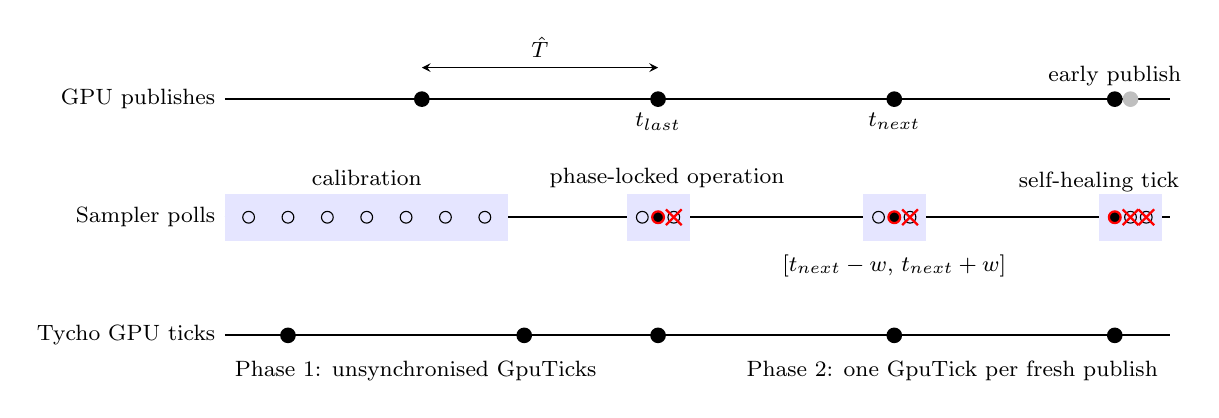
\begin{tikzpicture}[
    >=stealth,
    publish/.style={circle,fill=black,inner sep=2pt},
    poll-calib/.style={circle,draw=black,inner sep=1.5pt},
    poll-base/.style={circle,fill=black,inner sep=1.5pt},
    poll-burst/.style={circle,draw=black,inner sep=1.5pt},
    tick/.style={circle,fill=black,inner sep=2pt},
    timeline/.style={thick},
    label/.style={font=\footnotesize}
]

% Horizontal extents
\def\xmin{0}
\def\xmax{12}

% Y positions for the three lanes
\def\ygpu{3.2}
\def\ysampler{1.7}
\def\ytick{0.2}

% ------------------------------------------------------------------
% 1) GPU publish lane (ground truth)
% ------------------------------------------------------------------
\draw[timeline] (\xmin,\ygpu) -- (\xmax,\ygpu);
\node[label,anchor=east] at (\xmin,\ygpu) {GPU publishes};

% True publish events (roughly equidistant), last one early at 11.3
\foreach \x in {2.5,5.5,8.5} {
  \node[publish] at (\x,\ygpu) {};
}

% Actual early publish
\node[publish] at (11.3,\ygpu) {};
\node[label,anchor=south] at (11.3,\ygpu+0.05) {early publish};

% Expected publish (ghost marker) at 11.5
\node[circle,fill=gray!50,inner sep=2pt] at (11.5,\ygpu) {};

% Annotate approximate period between two publishes
\draw[<->] (2.5,\ygpu+0.4) --
    node[label,above] {$\hat{T}$}
    (5.5,\ygpu+0.4);

% Mark t_last and t_next for illustration
\node[label,anchor=north] at (5.5,\ygpu-0.05) {$t_{\text{last}}$};
\node[label,anchor=north] at (8.5,\ygpu-0.05) {$t_{\text{next}}$};

% ------------------------------------------------------------------
% 2) Sampler lane (calibration + phase-locked polls with burst window)
% ------------------------------------------------------------------
\draw[timeline] (\xmin,\ysampler) -- (\xmax,\ysampler);
\node[label,anchor=east] at (\xmin,\ysampler) {Sampler polls};

% Calibration phase block (left)
\def\xcalibStart{0.0}
\def\xcalibEnd{3.6}
\fill[blue!10] (\xcalibStart,\ysampler-0.3) rectangle (\xcalibEnd,\ysampler+0.3);
\node[label] at ({0.5*(\xcalibStart+\xcalibEnd)},\ysampler+0.50) {calibration};

% Calibration-phase polls (irregular, more frequent)
\foreach \x in {0.3,0.8,1.3,1.8,2.3,2.8,3.3} {
  \node[poll-calib] at (\x,\ysampler) {};
}

% Burst-style windows around predicted publish times in phase-locked regime
\def\tpred{5.5}
\def\whalf{0.4}
\fill[blue!10] (\tpred-\whalf,\ysampler-0.3) rectangle (\tpred+\whalf,\ysampler+0.3);

\def\tpred{8.5}
\def\whalf{0.4}
\fill[blue!10] (\tpred-\whalf,\ysampler-0.3) rectangle (\tpred+\whalf,\ysampler+0.3);
\node[label,anchor=north] at (\tpred,\ysampler-0.35)
  {$[t_{\text{next}}-w,\,t_{\text{next}}+w]$};

\def\tpred{11.5}
\def\whalf{0.4}
\fill[blue!10] (\tpred-\whalf,\ysampler-0.3) rectangle (\tpred+\whalf,\ysampler+0.3);

% Phase-locked base polls: successful observation polls
\node[poll-base,draw=red,thick] at (5.5,\ysampler) {};
\node[poll-base,draw=red,thick] at (8.5,\ysampler) {};
% Last window: successful observation comes slightly early
\node[poll-base,draw=red,thick] at (11.3,\ysampler) {};
\node[label,anchor=south] at (11.1,\ysampler+0.2) {self-healing tick};

% Additional burst-mode polls around t_next (denser sampling inside window)
\foreach \x in {5.3,5.7,8.3,8.7,11.5,11.7} {
  \node[poll-burst] at (\x,\ysampler) {};
}

% Polls that get skipped AFTER a successful observation:
% - in the first two windows: the late burst poll
% - in the last window: the scheduled base poll at 11.5 and the late burst poll at 11.7
\foreach \x in {5.7,8.7,11.5,11.7} {
  \draw[red,thick] (\x-0.10,\ysampler-0.10) -- (\x+0.10,\ysampler+0.10);
  \draw[red,thick] (\x-0.10,\ysampler+0.10) -- (\x+0.10,\ysampler-0.10);
}

% Optional annotation: phase-locked region
\node[label,anchor=west] at (4.0,\ysampler+0.50) {phase-locked operation};

% ------------------------------------------------------------------
% 3) Tycho GPU tick lane (two phases)
% ------------------------------------------------------------------
\draw[timeline] (\xmin,\ytick) -- (\xmax,\ytick);
\node[label,anchor=east] at (\xmin,\ytick) {Tycho GPU ticks};

% Phase 1: same cadence as publishes, but not phase-aligned (during calibration)
\foreach \x in {0.8,3.8} {
  \node[tick] at (\x,\ytick) {};
}

% Phase 2: phase-locked, one tick per fresh device update
\foreach \x in {5.5,8.5,11.3} {
  \node[tick] at (\x,\ytick) {};
}

\node[label,anchor=west] at (0.0,\ytick-0.45)
  {Phase 1: unsynchronised \code{GpuTick}s};

\node[label,anchor=west] at (6.5,\ytick-0.45)
  {Phase 2: one \code{GpuTick} per fresh publish};

\end{tikzpicture}
\caption{Phase-aware GPU polling timeline}
\label{fig:gpu_phaseaware_timeline}
\end{figure}

\paragraph{Tick Semantics.}
A \code{GpuTick} is emitted only when Tycho detects a genuinely new hardware
update.  Each tick contains a snapshot of device-level metrics and, when
available, process-level utilisation aligned to the same monotonic timestamp.
This design ensures that GPU measurements participate in Tycho's
cross-domain correlation without interpolation, resampling, or ad hoc
realignment.  The one-to-one correspondence between hardware updates and GPU
ticks is a core architectural guarantee and the primary distinction between
Tycho's approach and traditional periodic sampling.

\paragraph{Process Telemetry Integration.}
Process-level metrics describe aggregated utilisation over a wall-clock window
that is defined by the backend rather than Tycho's timing engine.  The
architecture treats these windows as retrospective measurements that must be
aligned with the device timeline.  Each process record is anchored to the
timestamp of the device snapshot that triggered its acquisition.  This preserves
temporal coherence in spite of the retrospective semantics of process telemetry
and supports multi-tenant attribution across GPU workloads.

\paragraph{Integration with the Global Timing Model.}
All GPU ticks are timestamped using Tycho's global monotonic timebase and
inserted into the multi-domain ring buffer. This ensures strict temporal ordering
relative to RAPL, Redfish, and eBPF data.  The architecture maintains the
principle of domain autonomy: each subsystem generates updates according to its
own temporal behaviour, while the analysis engine later fuses these streams into
a consistent attribution result.

\paragraph{Architectural Limitations.}
Although the architecture abstracts over backend differences, several structural
constraints remain. Telemetry capabilities vary significantly across NVIDIA devices and driver
configurations.
Some accelerators expose high-quality instantaneous power fields and cumulative
energy counters, while others provide only averaged power and coarse utilisation.

The implicit publish cadence may drift under DVFS or thermal transitions, which
limits the predictability of update edges.  
Tycho mitigates these effects through robust sampling logic in the implementation,
but the fidelity of the resulting GPU timeline remains bounded by the behaviour
of the underlying hardware.

Overall, the GPU subsystem elevates accelerator telemetry to a first-class
component of Tycho's energy model.  By aligning sampling with the device's
publish behaviour and unifying device and process metrics under a single
timestamping model, the architecture enables precise, temporally consistent
attribution in heterogeneous accelerator environments.

\section{Metadata Collection Subsystem}
\label{sec:arch_metadata_collection}

Tycho treats workload identity as a first-class architectural concern that is
strictly separated from numerical telemetry.
While energy and utilisation collectors emit temporally ordered measurement
streams, metadata captures the structural relationships required to interpret
those streams during analysis.
This includes the association of processes, containers, and pods as they evolve
over the lifetime of a node.

Metadata is maintained as cached identity state rather than as a time series.
It is neither aggregated nor iterated over analysis windows and does not
participate directly in temporal correlation.
Instead, metadata provides a bounded, continuously refreshed snapshot of recent
workload structure that must remain sufficiently fresh and temporally consistent
to support later attribution.
Consequently, metadata collection prioritises controlled refresh and bounded
lifetime over high-frequency or event-level precision.

\paragraph{Subsystem overview.}
The metadata subsystem forms a dedicated architectural layer that operates
independently of metric collection and analysis.
It consists of a small set of autonomous collectors coordinated through a single
metadata controller, which constitutes the sole authority over metadata mutation
and lifecycle management.
Collectors observe the system independently, but all state updates are mediated
by the controller, enforcing a clear separation between identity acquisition and
subsequent analytical processing.

\paragraph{Dual-collector model.}
Workload identity is inherently multi-sourced.
Tycho therefore integrates two complementary metadata collectors, each providing
a partial and independently valid view of system state:
\begin{itemize}
  \item \textbf{proc-collector:} observes process identity, execution context, and
        cgroup membership directly from the Linux kernel via the filesystem
        interface, providing authoritative runtime state independent of
        orchestration abstractions.
  \item \textbf{kubelet-collector:} acquires namespace-, pod- and container-level identity from
        the Kubernetes node agent, exposing scheduling and lifecycle information
        unavailable at the operating-system level.
\end{itemize}
The metadata subsystem does not attempt to fuse or interpret these views at
collection time.
Instead, it records the most recent identity state observed by each source and
defers reconciliation to analysis-time logic.

\paragraph{Controller-based coordination and scheduling.}
Metadata collection in Tycho is explicitly \emph{analysis-driven}.
The start of an analysis cycle constitutes the primary trigger for metadata
refresh and is treated as the highest-priority collection opportunity.
When an analysis window begins, the analysis engine requests a best-effort
refresh of all registered metadata collectors in order to obtain the most recent
possible identity state.

Autonomous metadata collectors exist as a secondary mechanism whose sole purpose
is to bound metadata age when analysis intervals are long.
These collectors execute under controller supervision and are explicitly
subjugated to analysis-driven collection.
If an analysis-triggered refresh is imminent, periodic collectors are suppressed
and defer execution to the analysis engine, preventing redundant collection in
short succession.

All collectors register with a central metadata controller, which arbitrates
between analysis-triggered and background execution.
The controller tracks the timestamp of the most recent successful observation for
each collector and enforces source-specific freshness constraints.
Collection is permitted only when required to satisfy source-specific freshness
constraints. As a result, metadata may be refreshed multiple times within a single analysis
window under long-running analysis, while redundant collection near analysis
boundaries is suppressed to reduce overhead.

This prioritisation establishes a clear architectural guarantee.
Metadata is maximally fresh at analysis start, redundant collection is avoided,
and collection overhead remains bounded independently of both analysis frequency
and global scheduling cadence.


\paragraph{Metadata state and lifetime model.}
Collected metadata is stored in a dedicated in-memory state that represents a
bounded snapshot of recent workload identity.
Unlike the ring-buffer–based design used for metric data, the metadata store
retains only the most recent valid representation of each observed entity.
Entries correspond to identity-bearing objects such as processes, containers, and
pods and are keyed by stable identifiers.
New observations update entries in place; historical versions and event sequences
are not preserved beyond the lifetime of the buffer window.

Each metadata entry carries a monotonic timestamp anchored to Tycho’s global
timebase, allowing identity state to be interpreted consistently alongside energy
and utilisation measurements.
Metadata is considered valid from its most recent observation until it is removed
by lifecycle management.
Garbage collection is horizon-based and enforced exclusively by the controller,
which removes entries once they fall outside the retained temporal window.
Collectors never delete metadata directly, ensuring deterministic expiry and
consistent memory bounds.

By coupling metadata lifetime to a bounded horizon rather than to explicit
lifecycle events, the subsystem remains robust to incomplete or delayed
observations.
Terminated processes, containers, and pods persist only long enough to support
analysis windows and are removed automatically once they passt the removal horizon.

\section{Calibration}
\label{sec:calibration}

Calibration is an auxiliary architectural subsystem that bounds temporal
uncertainty introduced by hardware-controlled metric publication.
It exists to constrain polling behaviour and temporal alignment for metric
sources whose update cadence or observable reaction latency is externally
governed and not analytically predictable.
Calibration is applied selectively and only where such uncertainty significantly
affects the correctness of subsequent analysis.

Calibration produces static, conservative parameters that are consumed by the
timing and analysis subsystems.
It does not participate in runtime attribution, does not adapt dynamically, and
does not operate on live metric streams.
By resolving temporal uncertainty ahead of time, calibration allows the runtime
system to remain deterministic, bounded, and non-intrusive.

Tycho distinguishes two independent calibration concerns:
\emph{polling-frequency calibration}, which bounds how often a metric source must
be queried to avoid undersampling hardware updates, and \emph{delay calibration},
which bounds the latency between a workload transition and the first observable
reaction in a metric stream.
These concerns are orthogonal and are applied only where their respective
assumptions hold.

\paragraph{Polling-frequency calibration.}
Polling-frequency calibration applies to metric sources whose publish cadence is
hardware-controlled and approximately regular.
Its purpose is to derive a conservative polling interval that observes all
published updates under nominal conditions without imposing unnecessary
collection overhead.

Polling-frequency calibration is performed during Tycho startup.
It relies exclusively on passive observation of device behaviour and does not
require workload manipulation.
This calibration is applied to GPU and Redfish power metrics, whose firmware- or BMC-controlled publication intervals are stable in expectation but not analytically documented.
The resulting polling bounds are treated as configuration constraints by the
timing subsystem and remain fixed during normal operation.
For node-level execution, Tycho adopts the most conservative bound across all
contributing devices to ensure uniform temporal coverage.

Polling-frequency calibration is not applied to RAPL or eBPF.
RAPL energy counters update quasi-continuously at a granularity far below
Tycho’s sampling resolution, rendering undersampling architecturally irrelevant.
eBPF metrics are event-driven and decoupled from device-side publish cadence,
making polling-frequency discovery unnecessary.

\paragraph{Delay calibration.}
Delay calibration bounds the latency between a workload transition and the first
observable change in a metric stream.
This calibration applies only where such latency is stable, workload-independent,
and sufficiently repeatable to be treated as a bounded constant.

Delay calibration is performed exclusively for GPU power metrics.
GPU devices internally aggregate and buffer power readings prior to publication,
introducing a measurable and consistent delay relative to workload onset.
Accurate estimation of this delay requires the generation of controlled,
high-intensity workload transitions to elicit clear device responses.
As Tycho is architecturally constrained to non-intrusive observation, such
stimulus-driven measurement is performed offline and excluded from runtime
operation.
The resulting delay bounds are supplied as static configuration parameters and inform the analysis subsystem’s temporal alignment logic without participating in runtime attribution.

No delay calibration is performed for RAPL or eBPF.
At Tycho’s temporal resolution, residual access latency in RAPL energy counters
is negligible, and eBPF metrics reflect execution state transitions without
device-side buffering.
Both domains are therefore treated as temporally immediate at the architectural
level.

Delay calibration is not applied to Redfish.
Redfish power readings exhibit irregular publish intervals, variable network
latency, and opaque BMC-internal behaviour, precluding stable delay estimation.
Redfish metrics are consequently treated as coarse, low-resolution signals
suitable for slow global trends, with temporal consistency enforced through
separate freshness and scheduling mechanisms. Architecturally, calibration constrains admissible interpretation without introducing additional runtime state or adaptive behavior.


\section{Analysis and Attribution Architecture}
\label{sec:analysis_attribution_arch}

\subsection{Pipeline Orchestration and Stage Execution}
\label{sec:arch_analysis_orchestration}

\subsubsection{Problem Statement}
Tycho’s analysis layer must transform heterogeneous, asynchronous observations into window-scoped attribution results under three constraints.
Inputs originate from independent sources with bounded but non-uniform delays and may be temporarily unavailable.
Attribution further requires interdependent derived quantities, imposing strict ordering constraints.
Finally, analysis must remain online, deterministic, and non-retrospective, excluding retrospective reinterpretation and any semantic coupling to exporter behavior.
The orchestration problem is therefore to execute a deterministic, dependency-respecting transformation pipeline per attribution window while tolerating partial observability and enforcing the invariants defined in \S~\ref{subsec:window_construction}.

\subsubsection{Conceptual Model}
Analysis proceeds as a sequence of discrete \emph{cycles}.
Each cycle selects a single attribution window, instantiates a self-contained execution context, executes a fixed set of transformations in a predefined order, and yields a logically atomic set of window-scoped derived quantities.
The analysis engine acts solely as an orchestration authority.
It determines the temporal scope of each cycle using the global monotonic timebase, enforces execution order, and commits results as a coherent unit.
Collection, buffering, and metadata acquisition are upstream concerns and are assumed to have materialized raw observations into bounded-retention histories.

The pipeline is expressed as a set of \emph{metrics}, each representing a typed transformation.
Metrics consume raw observations or previously derived metrics and emit window-scoped results according to the semantic models defined in this chapter.
Metrics may depend on earlier outputs within the same cycle but never on downstream publication state or future cycles.

\subsubsection{Attribution Window Semantics}
\label{sec:arch_analysis_orchestration_windows}
Let \(t_k\) denote the monotonic timestamp associated with the start of analysis cycle \(k\).
The attribution window for cycle \(k\) is defined as the half-open interval
\begin{equation}
W_k = (t_{k-1},\, t_k] .
\end{equation}
Windows are defined on a global monotonic timebase, form a total order, and are non-overlapping.

Window selection incorporates a fixed intentional lag relative to real-time execution.
The window end \(t_k\) is chosen such that it lags the most recent observations by at least the maximum admissible metric delay plus a safety margin, derived from configuration and optional calibration (\S~\ref{sec:calibration}).
This bound is an architectural precondition for window validity and guarantees that all metrics participating in a cycle can interpret their contributions over \(W_k\) under their declared delay semantics.
As a result, attribution correctness is decoupled from collector jitter, speculative window closure is avoided, and causality is preserved.

In steady state, attribution windows have a fixed duration.
During startup, when insufficient history exists, the window start may be clamped to the beginning of the monotonic timeline.
This is the only permitted deviation from the steady-state definition and preserves determinism.

\subsubsection{Stage Model and Dependency Discipline}
\label{sec:arch_analysis_orchestration_stages}
Analysis is structured as an ordered sequence of conceptual stages reflecting semantic dependencies between derived quantities.
A stage delineates computations whose outputs serve as prerequisites for subsequent modeling or attribution steps.
Within a cycle, stages execute strictly in order.
Metrics may depend on raw observations and on outputs from earlier stages in the same cycle, but must not depend on later stages, future cycles, or sink side effects.

This discipline renders the pipeline compositional.
Later attribution logic operates on materialized, window-scoped quantities rather than ad hoc joins over raw histories.
Stages are semantic boundaries, not runtime entities, and exist to make dependency structure explicit when partial observability yields incomplete but internally consistent results.

Figure~\ref{fig:analysis-stage-pipeline} summarizes the conceptual staging of the analysis pipeline within a single attribution cycle, illustrating the ordering constraints, data dependencies, and source materialization underlying window-scoped attribution.

\begin{figure}[t]
  \centering
  \includegraphics[width=\textwidth]{Figures/drawio/tycho_analysis_stages.png}
  \caption{Conceptual staging of the analysis pipeline for a single attribution window.}
  \label{fig:analysis-stage-pipeline}
\end{figure}


\subsubsection{Best-Effort Semantics Under Partial Observability}
\label{sec:arch_analysis_orchestration_best_effort}
The analysis architecture is accuracy-first but not completeness-first.
For a given window, Tycho produces the most complete set of derived quantities that can be computed without violating architectural invariants.
If required inputs are unavailable or inadmissible under a metric’s semantics, that metric is undefined for the window and does not materialize a result.
Downstream metrics may still execute if their dependencies are satisfied, yielding partially populated but self-consistent outputs.
As observability decreases, results degrade monotonically through omission or explicitly defined fallback semantics, and previously valid interpretations are never revised.

\subsubsection{Output Commit and Sink Boundary}
\label{sec:arch_analysis_orchestration_commit}
All results produced during a cycle belong to the same attribution window \(W_k\) and are committed as a logical batch.
Sinks are strictly downstream observers and lie outside the correctness boundary of attribution.
Exporter behavior may delay or drop publication but does not affect the meaning of computed window-scoped quantities.
This separation prevents exporter mechanics from becoming an implicit part of attribution semantics and preserves reproducibility.

\subsubsection{Architectural Consequences}
The orchestration model establishes a stable execution contract.
Stage-local computations may assume a well-defined attribution window, deterministic ordering, and read-only access to upstream histories.
In return, analysis is constrained to be window-scoped and non-retrospective.
Each cycle yields a single, maximal, internally consistent interpretation of the evidence available for its window, and later cycles do not revise earlier results.
This contract supports the staged construction of increasingly sophisticated attribution models without altering orchestration semantics.

\subsection{Stage 1: Component Metric Construction}
\label{subsec:stage1_component_metrics}
This stage defines how raw observations emitted by the collectors are transformed into coherent per-component total energy and power metrics. Its purpose is to establish temporally aligned, conservation-preserving component signals from heterogeneous inputs, independent of any attribution or decomposition semantics. The resulting metrics form the authoritative total-energy basis for all subsequent stages and are exported as externally consumable component-level measurements.

\subsubsection{Component-Level eBPF Utilization Metrics}
\label{sec:arch_ebpf_util_metrics}

\paragraph{Problem Statement.}
eBPF exposes raw kernel execution signals and hardware event counts as per-tick deltas.
These signals must be transformed into window-aligned utilization metrics with well-defined semantics and into cumulative counters suitable for direct export and downstream aggregation.

\paragraph{Conceptual Model.}
Two classes of node-level metrics are constructed from eBPF observations.
CPU execution time is expressed as normalized time-share ratios over a fixed analysis window.
All other kernel and hardware signals are expressed as cumulative counters obtained by aggregating per-process deltas across the node.

\paragraph{Formalization.}
Let a node expose $C$ logical CPUs and let an analysis window of duration $\Delta t$ define a total schedulable capacity
\begin{equation}
T_{\mathrm{cap}} = C \cdot \Delta t .
\end{equation}
Let $T_{\mathrm{idle}}$, $T_{\mathrm{irq}}$, and $T_{\mathrm{softirq}}$ denote the aggregated CPU time spent in idle, hardware interrupt, and software interrupt execution over the window.
Normalized utilization ratios are defined as
\begin{equation}
r_x = \frac{T_x}{T_{\mathrm{cap}}}, \quad x \in \{\mathrm{idle}, \mathrm{irq}, \mathrm{softirq}\}.
\end{equation}
Active execution is defined as the residual
\begin{equation}
r_{\mathrm{active}} = 1 - (r_{\mathrm{idle}} + r_{\mathrm{irq}} + r_{\mathrm{softirq}}).
\end{equation}
By construction, all ratios are dimensionless, bounded in $[0,1]$, and satisfy
\begin{equation}
r_{\mathrm{idle}} + r_{\mathrm{irq}} + r_{\mathrm{softirq}} + r_{\mathrm{active}} = 1.
\end{equation}

For each kernel or hardware event type $j$, let $\Delta K_j$ denote the per-tick delta aggregated across all processes.
The exported counter is defined as the cumulative sum
\begin{equation}
N_j(t) = \sum_{k \le t} \Delta K_j ,
\end{equation}
which is monotonically non-decreasing over the lifetime of the process.

\paragraph{Design Decisions.}
CPU utilization is normalized to node capacity to make ratios invariant to window length and core count.
Active CPU time is defined as a residual to enforce exact conservation of CPU capacity.
All event-based metrics are exposed as cumulative counters to preserve monotonicity and allow rate derivation without reinterpreting window semantics.

\paragraph{Architectural Consequences.}
The resulting metrics provide window-stable CPU utilization ratios and strictly monotonic kernel activity counters.
These quantities can be consumed directly as observability metrics and reused unchanged by downstream attribution stages.

\subsubsection{RAPL Component Metrics}

\paragraph{Problem Statement.}
RAPL exposes cumulative energy counters per hardware domain, but these counters are node-local, socket-scoped, and offset by an arbitrary hardware-defined origin.
For Tycho, these signals must be transformed into a single, coherent component-level energy metric that is comparable across time and suitable as an authoritative input for later attribution stages.
The core problem is therefore to define a metric that preserves the physical meaning of RAPL energy while eliminating hardware-specific offsets and remaining stable under windowed analysis.

\paragraph{Conceptual Model.}
The RAPL component is modeled as a set of independent energy domains, treated as conceptually separate devices but belonging to the same component.
For each domain, Tycho constructs a cumulative energy signal that represents the total physical energy consumed since Tycho start.
This signal is defined independently of any windowing semantics and serves as the primary representation of RAPL energy within the system.
A secondary, auxiliary power signal is derived from the same observations for user-facing inspection, but it is not authoritative.

\paragraph{Formalization.}
Let $E_d^{\text{raw}}(t)$ denote the raw cumulative RAPL energy reading for domain $d$ at time $t$, as provided by the underlying measurement subsystem.
These raw counters are assumed to be strictly monotonic and already corrected for hardware wraparound.

For each domain $d$, Tycho defines an exported cumulative energy counter
\begin{equation}
E_d(t) = E_d^{\text{raw}}(t) - E_d^{\text{raw}}(t_0),
\end{equation}
where $t_0$ is the time of the first observed sample for that domain.
This construction yields a zero-based, monotonic energy counter with $E_d(t_0)=0$.

An auxiliary average power signal is defined over an analysis window $[t_i, t_{i+1}]$ as
\begin{equation}
P_d^{(i)} = \frac{E_d(t_{i+1}) - E_d(t_i)}{t_{i+1} - t_i}.
\end{equation}
This quantity is derived solely from the cumulative energy counter and has no independent physical authority.

\paragraph{Design Decisions.}
The primary design choice is to treat cumulative energy as the first-class metric and to derive all other quantities from it.
Using zero-based cumulative counters removes dependence on hardware-specific initial offsets and simplifies downstream reasoning.
Power is intentionally modeled as a derived, window-local quantity rather than as a primary signal, reflecting its lower robustness and its lack of necessity for attribution.
Domains are defined once and treated uniformly, avoiding domain-specific special cases in the metric definition.

\paragraph{Architectural Consequences.}
The exported RAPL energy counters form the authoritative energy input for all later attribution and decomposition stages.
Their monotonicity and zero-based semantics allow unambiguous differencing, aggregation, and conservation reasoning.
By contrast, the power metrics are explicitly auxiliary, non-authoritative, and excluded from downstream attribution logic.
This separation ensures that attribution correctness depends only on cumulative energy, while still permitting power-oriented inspection for diagnostic or user-facing purposes.

\subsubsection{GPU-Corrected Energy Metric}

\paragraph{Problem Statement.}
GPU telemetry provides multiple power- and energy-related observations of the same physical process under incompatible temporal semantics.
Instantaneous power samples, one-second averaged power values, and optional cumulative energy counters are reported concurrently but cannot be combined by direct integration or signal selection without introducing temporal bias or discarding information.
Using any single signal in isolation either preserves absolute correctness at coarse granularity or improves temporal resolution at the cost of systematic error.
The problem addressed here is therefore not measurement scarcity, but the absence of a principled method to reconcile redundant GPU observations into a single, temporally refined, internally consistent power and energy signal aligned to corrected time.

\paragraph{Conceptual Model.}
GPU power is modeled as a latent, non-negative, continuous-time signal reconstructed on a uniform corrected-time grid and maintained over a retained history horizon that exceeds the current analysis window.
This deliberate use of historical context is a central accuracy mechanism, allowing delayed, coarse, and partially redundant observations to be reconciled in a globally consistent manner that window-local estimation cannot achieve.
All raw GPU observations are interpreted as constraints on this latent signal, jointly shaping a single authoritative power timeline per device.
Instantaneous and one-second averaged power samples impose soft consistency constraints, while cumulative energy counters, when available, act as dominant anchors that strongly influence the reconstruction without enforcing hard equality.
Physical plausibility is enforced by penalizing implausible curvature while preserving total energy and long-term magnitude.
Windowed GPU energy and power metrics are obtained by integrating sub-intervals of this maintained reconstructed signal, ensuring temporal coherence across windows and improved accuracy relative to any raw observation stream.

\paragraph{Formalization.}
For each GPU device, power is represented by a reconstructed sequence
\( p = \{p_k\}_{k=0}^{N-1} \) on a uniform corrected-time grid with spacing \( \Delta t \).
Reconstruction is posed as a constrained optimization problem that minimizes weighted discrepancies to observed telemetry while enforcing physical plausibility.
Let \( \mathcal{R} \) denote the set of observation constraints derived from instantaneous power samples, one-second averaged power samples, and optional cumulative energy readings.
Each constraint \( r \in \mathcal{R} \) is expressed by a linear operator \( a_r \) acting on \( p \) with target value \( y_r \) and weight \( w_r \).

The architectural objective is
\begin{equation}
\min_{p \ge 0}
\;\sum_{r \in \mathcal{R}} w_r^2 \left(a_r^\top p - y_r\right)^2
\;+\;
\lambda_D \sum_{k=1}^{N-2}
\left(p_{k+1} - 2p_k + p_{k-1}\right)^2 ,
\end{equation}
where the second-difference term penalizes curvature without imposing a prior on absolute magnitude.
Non-negativity \( p_k \ge 0 \) enforces physical feasibility.
Cumulative energy observations contribute constraints whose weights dominate when present, prioritizing energy consistency over time without enforcing exact equality.
The solution \( p \) defines the authoritative GPU power signal; windowed GPU energy is obtained by integrating \( p \) over the corresponding corrected-time interval.

\paragraph{Design Decisions.}
Constrained reconstruction is chosen over signal selection to avoid privileging any single telemetry source and to preserve all available information.
Cumulative energy counters are treated as dominant but soft constraints to exploit their reliability while tolerating gaps, resets, and delayed reporting.
Instantaneous and averaged power samples are retained as complementary observations that improve temporal resolution and stabilize reconstruction when energy counters are absent.
Smoothness is imposed via second differences to suppress implausible oscillations without biasing total energy or sustained power level.
No magnitude prior is introduced, as any bias toward lower power would conflict with the accuracy-first objective.
Numerical conditioning and solver-specific stabilization are intentionally excluded from the architectural model.

\paragraph{Architectural Consequences.}
The architecture yields a single corrected GPU power signal per device that is temporally finer than any raw input and internally consistent across power and energy representations.
All downstream GPU metrics are derived exclusively from this reconstructed signal, eliminating ambiguity from heterogeneous telemetry.
Historical retention becomes a first-class correctness mechanism, enabling stable, coherent windowed estimates under delayed and coarse observation regimes.
The design explicitly acknowledges the modeled nature of the result while guaranteeing physical plausibility and maximal energy consistency given available observations, establishing a stable foundation for subsequent attribution and aggregation stages.

\subsubsection{Redfish-Corrected System Energy Metric}
\label{sec:metric_redfish_arch}

\paragraph{Problem Statement.}
Raw Redfish power telemetry is sparse, irregular, and subject to delay that can vary over time.
Direct window integration of held power values yields a valid low-rate estimate, but it cannot provide temporally granular system power that is consistent across windows when sample timing drifts.
A second construction is therefore required that treats Redfish as the authoritative system-level anchor while reconstructing a higher-rate system power trajectory from contemporaneous component-proxy signals.

\paragraph{Conceptual Model.}
The metric family exports a canonical system power series and its cumulative energy counter, parameterized by a `source` label.
During warmup or when insufficient Redfish anchoring is available, \code{source="redfish\_raw"} is formed by integrating the held Redfish power trajectory.
Once sufficient Redfish observations exist over a reconstruction horizon, \code{source="redfish\_corrected"} replaces the raw series and represents a reconstructed system power trajectory on a fine time grid.
Reconstruction is posed as fitting a non-negative linear combination of proxy signals that are expected to co-vary with system power, while strongly anchoring the fit to the observed Redfish samples.

\paragraph{Formalization.}
Let $p_{\mathrm{RF}}(t)$ denote Redfish-reported system power (in mW), observed at irregular raw times $t^{\mathrm{raw}}_j$.
Redfish observations are subject to an unknown, time-varying reporting delay.
The construction therefore introduces an explicit delay parameter $\delta_{\mathrm{RF}} \ge 0$, mapping raw timestamps into a corrected domain
\begin{equation}
t_j = t^{\mathrm{raw}}_j - \delta_{\mathrm{RF}} .
\end{equation}

For the raw series, $p_{\mathrm{raw}}(t)$ is defined as a zero-order-hold trajectory of $p_{\mathrm{RF}}(t)$ in corrected time.
For an analysis window $W = [t_s, t_e]$ of duration $\Delta_W$ seconds, the window energy and average power are
\begin{equation}
E_{\mathrm{raw}}(W) = \int_{t_s}^{t_e} p_{\mathrm{raw}}(t)\, dt,
\qquad
P_{\mathrm{raw}}(W) = \frac{E_{\mathrm{raw}}(W)}{\Delta_W}.
\end{equation}

For the corrected construction, system power is reconstructed on a uniform grid of bins $k$ with width $\Delta$ milliseconds over a finite horizon.
Let $p_{\mathrm{hat}}[k]$ denote reconstructed system power in bin $k$.
For each bin, proxy features are derived from contemporaneous component metrics:
average package, DRAM, and GPU powers $p_{\mathrm{pkg}}[k]$, $p_{\mathrm{dram}}[k]$, $p_{\mathrm{gpu}}[k]$, and the CPU instruction rate $r_{\mathrm{instr}}[k]$.

Redfish observations are projected into the corrected domain at times $t_j$ and interpreted as constraints on the reconstruction
(optionally corresponding to a trailing-average kernel over a fixed interval).
Let $y_j$ denote the Redfish power value associated with observation $j$.
Reconstruction fits parameters $\theta = (\alpha,\beta,\gamma,\delta,b)$ such that
\begin{equation}
p_{\mathrm{hat}}[k] =
\max\!\left(
0,\,
\alpha\,p_{\mathrm{pkg}}[k]
+ \beta\,p_{\mathrm{dram}}[k]
+ \gamma\,p_{\mathrm{gpu}}[k]
+ \delta\,r_{\mathrm{instr}}[k]
+ b
\right),
\end{equation}
where $\alpha,\beta,\gamma,b \ge 0$ enforce physical non-negativity.

Crucially, $\delta_{\mathrm{RF}}$ is not fixed.
For each analysis cycle, a finite candidate set of delays is evaluated, and the delay is selected that minimises the unexplained system power
relative to the proxy sum over recent bins, subject to stability constraints.
This adaptive delay selection aligns Redfish observations to the proxy domain in a best-effort sense and is recomputed as system behaviour changes.

Window energy and power for the corrected series are obtained by integrating $p_{\mathrm{hat}}$ over the overlap of $W$ with the reconstruction grid:
\begin{equation}
E_{\mathrm{corr}}(W) = \int_{t_s}^{t_e} p_{\mathrm{hat}}(t)\, dt,
\qquad
P_{\mathrm{corr}}(W) = \frac{E_{\mathrm{corr}}(W)}{\Delta_W}.
\end{equation}

\paragraph{Design Decisions.}
Redfish is treated as the system-level anchor rather than as a weak label, so the fit objective is defined in observation space and evaluated only where Redfish provides constraints.
Delay is treated as an explicit degree of freedom in the construction because raw Redfish timestamps are not sufficient to guarantee stable alignment.
Proxy features are restricted to quantities that are already available at fine granularity, enabling reconstruction without introducing additional sensors.
Non-negativity constraints on physically interpretable coefficients prevent the model from compensating Redfish irregularities by introducing negative component contributions or a negative baseline.

\paragraph{Architectural Consequences.}
The construction yields a single canonical system series that remains available during warmup via \code{source="redfish\_raw"} and transitions to a higher-rate anchored estimate via \code{source="redfish\_corrected"} without changing metric IDs.
Downstream stages can treat the corrected series as the system-level power baseline for further decomposition, while retaining the provenance of the construction through the `source` label.
The reconstruction is intentionally conservative: when anchoring observations are insufficient or alignment is unreliable, corrected output is withheld and raw integration remains authoritative.

\subsection{Stage 2: System-Level Energy Model and Residual}
\label{subsec:stage2_residual}

\paragraph{Problem Statement.}
After Stage~1, Tycho provides multiple component-level energy signals that are individually conservative but incomplete.
No combination of RAPL and GPU measurements can fully account for total node energy consumption, and a system-level reference is required to constrain attribution.
While a window-aligned, system-wide energy signal can be constructed from Redfish telemetry, it represents only total consumption and cannot be decomposed into all contributing subsystems.
This creates a structural gap between modeled components and total system energy that must be addressed explicitly.

\paragraph{Conceptual Model.}
Stage~2 introduces a system-level energy balance scoped to a single node and a single analysis window.
Total system energy is taken from the integrated Redfish signal, while accounted component energy is defined as the sum of all explicitly modeled contributors.
Any remaining energy is captured explicitly as a residual term, representing unmodeled components and aggregation effects rather than measurement error.
Residual energy is therefore treated as a first-class quantity within the attribution pipeline.

\paragraph{Formalization.}
Let $E_{\text{sys}}$ denote total system energy for a window, obtained from the system-level source.
Let $E_{\text{parts}}$ denote the sum of all explicitly modeled component energies for the same window.
In this stage, $E_{\text{parts}}$ comprises the cumulative CPU package energy (including associated DRAM domains where available) and the sum of all GPU energy contributions, consistent with standard RAPL domain boundaries.
The residual energy $E_{\text{res}}$ is defined as:
\begin{equation}
E_{\text{res}} = E_{\text{sys}} - E_{\text{parts}}.
\end{equation}
This definition is local to a node and window and does not imply workload attribution.
The architectural invariant enforced by Stage~2 is strict energy conservation at the window level.

\paragraph{Design Decisions.}
Residual energy is modeled explicitly rather than absorbed into noise or redistributed across components.
This avoids introducing hidden assumptions about unmodeled hardware behavior and preserves auditability.
Temporal misalignment between system and component signals is tolerated at the power level but never allowed to violate energy conservation.
No attempt is made at this stage to reinterpret or smooth the residual term.

\paragraph{Architectural Consequences.}
Stage~2 establishes a closed system-level energy budget that constrains all downstream attribution.
Later stages may further decompose or attribute residual energy, but they cannot eliminate it without introducing additional assumptions.
The explicit residual also enables the system to signal when residual-based interpretation is unreliable, without compromising conservation.

\subsection{Stage 3: Idle and Dynamic Energy Semantics}
\label{subsec:stage3_idle_dynamic}
This stage defines how total component energy is partitioned into idle and dynamic contributions prior to attribution. Because CPU packages, residual system energy, and GPUs differ in observability, baseline stability, and utilization coupling, the decomposition semantics are specified per component rather than uniformly. The following subsubsections formalize these component-specific rules while preserving energy conservation and temporal consistency, and while establishing dynamic signals suitable for downstream attribution. Each decomposition defined below follows the same architectural pattern: a conservative baseline definition, a non-negative dynamic remainder obtained by conservation, and explicit admissibility conditions that bound when the resulting quantities may be interpreted.

\subsubsection{RAPL Idle and Dynamic Decomposition}
\label{sec:arch_rapl_idle_dynamic}

\paragraph{Problem Statement.}
RAPL exposes per-domain total energy that merges baseline platform consumption with workload-induced variation.
For attribution and downstream fairness policies, Tycho requires a conservative split into an approximately stable idle component and a residual dynamic component while preserving per-window energy conservation.

\paragraph{Conceptual Model.}
For each RAPL domain $d \in \{\code{pkg},\code{core},\code{uncore},\code{dram}\}$, Tycho treats the exported total power $P^{\mathrm{tot}}_d(t)$ as the sum of an idle baseline $P^{\mathrm{idle}}_d(t)$ and a dynamic remainder $P^{\mathrm{dyn}}_d(t)$.
Idle is estimated from low-activity operating points using an external utilization proxy $u_d(t)$ and a model that targets the theoretical $u_d=0$ intercept, avoiding reliance on observing a true zero-load system.
This preference follows the empirical finding that linear models yield robust idle estimates while higher-order fits tend to be unreliable in practice \parencite{pijnackerContainerlevelEnergyObservability2025}.

\paragraph{Formalization.}
Let $W_k$ denote an analysis window of duration $\Delta t_k$ and let $\Delta E^{\mathrm{tot}}_{d,k}$ be the total domain energy increment over $W_k$.
Tycho defines the decomposition by a baseline power estimate $\beta_{d,k}$ and constructs window energies as:
\begin{equation}
\Delta E^{\mathrm{idle}}_{d,k} = \min\!\left(\Delta E^{\mathrm{tot}}_{d,k},\; \max(0,\beta_{d,k}) \cdot \Delta t_k \right),
\end{equation}
\begin{equation}
\Delta E^{\mathrm{dyn}}_{d,k} = \Delta E^{\mathrm{tot}}_{d,k} - \Delta E^{\mathrm{idle}}_{d,k}.
\end{equation}
The baseline $\beta_{d,k}$ is obtained by fitting a linear model $P^{\mathrm{tot}}_d \approx \alpha_d u_d + \beta_d$ using only samples drawn from stable, low-utilization regimes and evaluating the intercept $\beta_d$ as the idle estimate.

\paragraph{Design Decisions.}
Tycho adopts utilization-conditioned estimation rather than pure lower-bound tracking to remain meaningful on continuously active Kubernetes nodes where true idle is rarely observed.
Model fitting is restricted to low-utilization operating points to prioritise identifiability of the intercept and avoid distortion by high-load regimes.
The decomposition is defined per RAPL domain, permitting distinct baselines for domains whose activity sensitivity differs.
Conservative clamping enforces non-negativity and prevents idle from exceeding total within a window, ensuring that the decomposition cannot create energy.

\paragraph{Architectural Consequences.}
The resulting per-domain $(\Delta E^{\mathrm{idle}}_{d,k}, \Delta E^{\mathrm{dyn}}_{d,k})$ split provides a stable baseline for policy-driven idle allocation while reserving fine-grained attribution capacity for the dynamic remainder.
Energy conservation holds per window by construction, enabling downstream stages to distribute dynamic energy without ambiguity and to route any non-attributable portions explicitly to the system bucket.

\subsubsection{Residual Idle and Dynamic Decomposition}

\paragraph{Problem Statement.}
Residual energy is defined as the portion of system-level energy not explained by explicitly modeled components.
While this residual budget is energy-consistent by construction, its instantaneous power signal is affected by temporal misalignment and measurement latency.
As a result, residual power cannot be interpreted uniformly across analysis windows.
A decomposition is required that preserves conservation of the residual budget while preventing transient artifacts from corrupting persistent state or downstream learning.

\paragraph{Conceptual Model.}
The residual budget is decomposed into two modeled components: a residual idle component and a residual dynamic component.
Residual idle represents a persistent, low-variance baseline within the residual budget, while residual dynamic captures the remaining window-local variation.
The decomposition is explicitly conditional.
Its semantic validity depends on a window usability predicate that identifies windows dominated by temporal misalignment.
When this predicate is false, the decomposition remains defined but must not be interpreted or used for learning.

\paragraph{Formalization.}
Let \( P^{\mathrm{res}}_w \) denote the non-negative residual total power for window \( w \).
For every window satisfying the usability predicate, the residual decomposition is defined as:
\begin{equation}
P^{\mathrm{res}}_w = P^{\mathrm{res,idle}}_w + P^{\mathrm{res,dyn}}_w
\end{equation}
with the invariants:
\begin{equation}
P^{\mathrm{res,idle}}_w \ge 0,\qquad
P^{\mathrm{res,dyn}}_w \ge 0,\qquad
P^{\mathrm{res,idle}}_w \le P^{\mathrm{res}}_w
\end{equation}

Residual idle power is defined using a persistent modeled baseline \( B^{\mathrm{res}} \):
\begin{equation}
P^{\mathrm{res,idle}}_w = \min\left(B^{\mathrm{res}}, P^{\mathrm{res}}_w\right)
\end{equation}
Residual dynamic power is defined by conservation:
\begin{equation}
P^{\mathrm{res,dyn}}_w = P^{\mathrm{res}}_w - P^{\mathrm{res,idle}}_w
\end{equation}

The interpretive contract of this decomposition holds only when the window usability predicate is true.
No fallback semantics are defined when this condition is violated.

\paragraph{Design Decisions.}
Residual idle is modeled as a persistent baseline rather than a per-window estimate.
This choice prevents transient measurement artifacts from collapsing the baseline and destabilizing downstream stages.
The model deliberately avoids any physical interpretation of residual idle or dynamic components.
By enforcing exact conservation and non-negativity, the decomposition remains bounded and conservative under all conditions.

\paragraph{Architectural Consequences.}
This decomposition provides a stable internal structure over unmodeled energy while explicitly limiting its semantic scope.
Downstream stages may rely on residual idle and dynamic quantities only when window usability is asserted.
At the same time, the model constrains interpretation by requiring consumers to treat usability as a hard semantic gate rather than a soft quality indicator.

\subsubsection{GPU Idle and Dynamic Decomposition}
\label{sec:arch_gpu_idle_dynamic}

\paragraph{Problem Statement.}
The corrected GPU power signal contains both an idle baseline and workload-induced dynamic consumption.
For attribution and energy accounting, Tycho must separate these components such that idle reflects the lowest sustainably attainable device power under low utilization, while dynamic captures the residual induced by activity.
This separation must be defined per device, since baseline power differs across GPUs and operating conditions.

\paragraph{Conceptual Model.}
For each GPU device identified by $\mathit{uuid}$, Tycho maintains an idle power estimate $\beta_{\mathit{uuid}}$ derived from the corrected total power signal under low and stable utilization.
The dynamic power is defined as the non-negative residual between total and idle.
Idle and dynamic energy increments are obtained by applying the same window duration used for the corresponding total power observation, ensuring that the decomposition is temporally consistent within each window.

\paragraph{Formalization.}
Let $P_{\mathit{uuid}}(w)$ denote the corrected total GPU power associated with analysis window $w$, and let $\beta_{\mathit{uuid}}(w)$ denote the idle power estimate available for that window.
Tycho defines the power decomposition as
\begin{equation}
P^{\mathrm{idle}}_{\mathit{uuid}}(w) = \mathrm{clip}\!\left(\beta_{\mathit{uuid}}(w),\, 0,\, P_{\mathit{uuid}}(w)\right),
\end{equation}
\begin{equation}
P^{\mathrm{dyn}}_{\mathit{uuid}}(w) = \max\!\left(0,\, P_{\mathit{uuid}}(w) - P^{\mathrm{idle}}_{\mathit{uuid}}(w)\right).
\end{equation}
With window duration $\Delta t(w)$, the corresponding per-window energy increments are
\begin{equation}
\Delta E^{\mathrm{idle}}_{\mathit{uuid}}(w) = P^{\mathrm{idle}}_{\mathit{uuid}}(w)\,\Delta t(w),
\end{equation}
\begin{equation}
\Delta E^{\mathrm{dyn}}_{\mathit{uuid}}(w) = P^{\mathrm{dyn}}_{\mathit{uuid}}(w)\,\Delta t(w).
\end{equation}
The decomposition is conservative by construction:
\begin{equation}
\Delta E^{\mathrm{idle}}_{\mathit{uuid}}(w) + \Delta E^{\mathrm{dyn}}_{\mathit{uuid}}(w) = P_{\mathit{uuid}}(w)\,\Delta t(w),
\end{equation}
up to discretization and clipping effects, and with all terms constrained to be non-negative.

\paragraph{Design Decisions.}
Tycho derives $\beta_{\mathit{uuid}}$ from the corrected power signal rather than raw device telemetry to preserve temporal consistency with the exported total power and to avoid bias from known sampling and delay artifacts.
Idle estimation is gated by stability of recent utilization observations and restricted to low-utilization regimes to prevent transient load onsets from being absorbed into the baseline.
The model is defined per device to avoid cross-GPU coupling and to allow heterogeneous baselines within the same node.

\paragraph{Architectural Consequences.}
Downstream stages may treat $(P^{\mathrm{idle}}_{\mathit{uuid}}, P^{\mathrm{dyn}}_{\mathit{uuid}})$ and their cumulative energies as a stable, non-negative decomposition of corrected total power per device.
The stability gate implies that $\beta_{\mathit{uuid}}$ evolves only under sufficiently stationary conditions, so dynamic power absorbs short-lived transients by default.
This design intentionally prioritizes robustness of the idle baseline over rapid adaptation to changing operating points.

\subsection{Stage 4: Workload Attribution and Aggregation}
\label{subsec:stage4_workload_attrib}
Stage 4 realises workload-level attribution by mapping system- and component-level signals to concrete execution contexts. It defines the admissible scope of attribution, resolves workload identity under partial observability, and materialises utilization metrics and CPU and GPU energy at the workload level, while explicitly bounding what is not attributed.

\subsubsection{Workload Resolution and the \code{\_\_system\_\_} Class}

\paragraph{Problem Statement.}
Energy signals observed by Tycho are not intrinsically associated with Kubernetes workloads.
Attribution therefore requires an explicit resolution step that maps low-level execution identities to container, pod, and namespace labels.
This mapping is inherently partial, asynchronous, and failure-prone due to process churn, PID reuse, delayed metadata visibility, and non-Kubernetes activity.
An architectural treatment is required to ensure that attribution remains total, conservative, and interpretable under these conditions.

\paragraph{Conceptual Model.}
Stage~4 operates on energy quantities that are already temporally aligned and semantically classified (total, idle, dynamic).
Workload attribution is defined as a conditional labeling step that associates each attributable energy portion with a Kubernetes workload identity when such an identity can be resolved with sufficient confidence.
Resolution is based on a best-effort join between execution-level observations and a metadata view that reflects the current Kubernetes state.
Energy portions for which no workload identity can be resolved are assigned to a distinguished workload class, denoted \code{\_\_system\_\_}, which represents non-attributable, infrastructural, or unresolved activity.

\paragraph{Formalization and Invariants.}
Let $E$ denote an energy quantity produced by earlier stages and let $\mathcal{W}$ be the set of resolvable Kubernetes workload identities.
Workload attribution defines a partial mapping $f : E \rightarrow \mathcal{W}$.
To preserve totality, this mapping is extended to a total function $\hat{f} : E \rightarrow \mathcal{W} \cup \{\code{\_\_system\_\_}\}$ by assigning all unresolved energy to \code{\_\_system\_\_}.
The following invariants hold for all Stage~4 outputs:
(i) conservation: the sum of workload-attributed energy equals the input energy,
(ii) non-negativity: no workload receives negative energy,
(iii) monotone degradation: loss of metadata resolution increases the share attributed to \code{\_\_system\_\_} but never reallocates energy between resolved workloads.

\paragraph{Design Decisions.}
The \code{\_\_system\_\_} label is treated as a first-class workload class rather than an absence of labeling.
This avoids silent energy loss, preserves comparability across runs with different metadata quality, and makes unresolved attribution explicit.
Workload resolution is deliberately decoupled from the attribution mathematics itself: the attribution model consumes resolved identities as inputs but does not embed resolution logic into its equations.
This separation ensures that attribution correctness degrades conservatively under partial observability.

\paragraph{Architectural Consequences.}
All workload-attributed metrics in Stage~4 share a common resolution boundary and a uniform interpretation of unattributable energy.
Metric-specific attribution logic may differ in how energy is distributed among resolved workloads, but unresolved energy is always surfaced explicitly via \code{\_\_system\_\_}.
This abstraction enables consistent downstream analysis while preventing speculative attribution beyond what the available metadata supports.

\subsubsection{Attribution Goals, Admissible Degrees of Freedom, and Temporal Granularity}

\paragraph{Problem Statement.}
Even when workload identities are available, distributing energy among workloads is fundamentally underdetermined.
Energy signals originate from shared components, while explanatory signals (utilization, activity, requests) are incomplete, indirect, and metric-specific.
An architectural framing is required that defines what attribution must guarantee, what it may choose freely, and where Tycho deliberately refrains from speculative precision.

\paragraph{Attribution Goals and Invariants.}
Stage~4 attribution is governed by a small set of global goals that apply uniformly across metrics.
Attribution must conserve energy, remain non-negative, and be complete over the workload domain extended by \code{\_\_system\_\_}.
Attribution must not retroactively reinterpret past decisions and must degrade monotonically under loss of explanatory signals.
Beyond these invariants, attribution is explicitly not required to recover a unique or physically exact decomposition.

\paragraph{Admissible Degrees of Freedom.}
Within these constraints, Tycho allows metric-specific definitions of \emph{fairness}.
A metric may distribute energy proportionally to observed activity, declared resource requests, or other admissible proxies, provided that the global invariants are preserved.
Fallback rules are permitted when proxies are missing or ill-defined, but such fallbacks must be explicit and must not introduce hidden redistribution between resolved workloads.
This separation allows each metric to encode its own fairness assumptions without contaminating the shared attribution framework.

\paragraph{Fine-Grained Temporal Attribution as a Core Principle.}
A defining architectural choice of Tycho is that attribution is performed at the finest temporal granularity supported by the underlying signal, prior to any window-level aggregation.
Energy portions are first attributed to workloads at this fine granularity and only then aggregated over the analysis window.
This design enables Tycho to distinguish workloads with different energy characteristics even when their aggregate utilization within a window is similar.
In contrast to window-pooled attribution schemes, this approach preserves temporal structure as an explanatory signal and avoids conflating heterogeneous workload behavior.

\paragraph{Architectural Consequences.}
Stage~4 defines attribution as a constrained optimization problem with explicit degrees of freedom rather than a fixed formula.
Metric-specific attribution sections instantiate these freedoms while inheriting the same invariants and temporal discipline.
As a result, Tycho can express nuanced workload energy differentiation when supported by data, while remaining conservative and interpretable when it is not.

\subsubsection{Explicit Non-Attribution of Redfish Metrics}

Redfish provides system-level power measurements that lack reliable workload-level explanatory signals.
Attributing these measurements to Kubernetes workloads would therefore require speculative assumptions about the contribution of individual activities to shared components such as memory subsystems, interconnects, storage, or firmware-controlled behavior.
Such assumptions are incompatible with Tycho’s accuracy-first design philosophy.

Consequently, Redfish metrics are excluded from Stage~4 workload attribution.
They are neither distributed across workloads nor labeled with \code{\_\_system\_\_} identities.
Instead, Redfish metrics remain system-scoped signals that may be used for validation, bounding, or cross-checking of attributed energy, but not as sources of workload-resolved energy data.

This exclusion is a deliberate architectural decision rather than a limitation of the implementation.
It preserves semantic clarity of workload-attributed metrics and prevents the introduction of unverifiable attribution artifacts.

\subsubsection{Workload Attribution of eBPF Utilization Counters}

\paragraph{Problem Statement.}
Fine-grained execution activity signals collected via eBPF are emitted at process scope and are not intrinsically associated with Kubernetes workloads.
To support workload-level analysis, these signals must be attributed to workload identities without modeling assumptions, while preserving conservation, non-negativity, and monotone degradation under partial observability.
Unlike energy signals, eBPF counters represent directly observed activity and therefore admit attribution by aggregation rather than distribution, but only if unresolved activity is handled explicitly and conservatively.

\paragraph{Conceptual Model.}
Each eBPF utilization signal is treated as a stream of per-process activity deltas observed at high temporal resolution.
Stage~4 attribution maps each process delta to a workload identity when resolution succeeds, and otherwise assigns it to a distinguished \code{\_\_system\_\_} workload class.
Workload-level utilization is obtained by summing all resolved process deltas per workload, while \code{\_\_system\_\_} captures the residual activity not attributable to any resolved workload.
No reweighting, normalization, or inference across workloads is performed.

\paragraph{Formalization.}
Let $\Delta u_p(t)$ denote the utilization delta of process $p$ over an attribution interval at time $t$, and let $R(p,t)$ be the workload resolution function, which yields either a workload $w$ or $\varnothing$.

The workload-attributed utilization $U_w(t)$ is defined as
\begin{equation}
U_w(t) = \sum_{p \mid R(p,t)=w} \Delta u_p(t),
\end{equation}
and the system residual is defined by construction as
\begin{equation}
U_{\code{\_\_system\_\_}}(t) =
\sum_p \Delta u_p(t) - \sum_{w \neq \code{\_\_system\_\_}} U_w(t).
\end{equation}
This definition guarantees conservation, completeness, and non-negativity, independent of resolution success.

\paragraph{Design Decisions.}
Utilization attribution is realized as aggregation rather than proportional distribution, reflecting that eBPF counters already encode directly attributable activity.
The \code{\_\_system\_\_} workload is defined as a residual class by construction rather than as a fallback resolution outcome, ensuring that all unresolvable activity is captured without bias toward resolved workloads.
Alternative schemes that discard unresolved activity or redistribute it among workloads were rejected due to violation of conservation and monotone degradation requirements.

\paragraph{Architectural Consequences.}
The resulting workload-level utilization counters form a complete and conservative attribution surface for execution activity.
They are directly comparable across workloads and over time, and remain interpretable under partial observability.
These metrics provide the explanatory substrate required for energy attribution analysis and validation, without introducing additional modeling assumptions or temporal coupling.

\subsubsection{CPU Dynamic Energy Attribution}

\paragraph{Problem Statement.}
CPU dynamic energy is exposed only as an aggregate per-domain signal for each RAPL CPU domain (\code{pkg}, \code{core}, \code{uncore}, \code{dram}) and is not intrinsically associated with individual workloads.
At the same time, workload activity is observable only indirectly through execution-level proxies with finite resolution and partial coverage.
The core problem is therefore to distribute a domain-level dynamic energy budget across workloads in a way that is conservative, temporally faithful, and robust to incomplete observability, while ensuring that attribution degrades monotonically toward the \code{\_\_system\_\_} class rather than redistributing energy among resolved workloads.

\paragraph{Conceptual Model.}
For a given analysis window $W$ and RAPL domain $B$, the authoritative input is the window-level dynamic energy budget $\Delta E_{B,\mathrm{dyn}}(W)$.
Attribution proceeds at native eBPF bin resolution and follows a two-stage model.
First, the window-level energy budget is distributed across fine-grained temporal bins proportionally to observed CPU activity in each bin.
Second, each bin’s energy share is distributed across workloads proportionally to their activity within that bin.
This preserves temporal structure as an explanatory signal while ensuring that attribution decisions are local to each bin and degrade conservatively when activity proxies are absent.

\paragraph{Formalization.}
Let $b \in W$ index the 50\,ms bins contained in window $W$.
For a given domain $B$, let $T_B(b)$ denote the total activity mass observed in bin $b$, and let $W_B(\ell,b)$ denote the activity mass attributed to workload $\ell$ in bin $b$.
The per-bin energy share is defined as
\begin{equation}
\Delta E_{B}(b) =
\begin{cases}
\Delta E_{B,\mathrm{dyn}}(W)\cdot \dfrac{T_B(b)}{\sum_{b' \in W} T_B(b')} & \text{if } \sum_{b' \in W} T_B(b') > 0, \\
0 & \text{otherwise}.
\end{cases}
\end{equation}
Within each bin, workload attribution is defined as
\begin{equation}
\Delta E_{B}(\ell,b) =
\begin{cases}
\Delta E_{B}(b)\cdot \dfrac{W_B(\ell,b)}{T_B(b)} & \text{if } T_B(b) > 0, \\
0 & \text{otherwise}.
\end{cases}
\end{equation}
If either $\sum_{b} T_B(b)=0$ or $T_B(b)=0$ for a given bin, the corresponding energy mass is assigned to the \code{\_\_system\_\_} workload, preserving completeness and conservation.

\paragraph{Design Decisions.}
Observed CPU activity is used as the sole fairness basis.
For the \code{pkg}, \code{core}, and \code{uncore} domains, activity is measured via per-process retired instruction counts.
For the \code{dram} domain, activity is measured via cache-miss counts, with a window-scoped fallback to CPU cycle counts when cache-miss mass is zero but cycle mass is non-zero.
This choice reflects the closest available causal relationship between workload behavior and domain-specific dynamic energy, while remaining explicit and conservative under missing signals.

\paragraph{Architectural Consequences.}
The resulting attribution is causal, temporally fine-grained, and strictly conservative.
All dynamic CPU energy is assigned either to resolved workloads or to \code{\_\_system\_\_}, with no redistribution between workloads under metadata loss.
The bin-level structure remains an explicit part of the architectural contract, enabling later extensions such as non-linear attribution rules or idle–dynamic decomposition without revisiting the core attribution model.

\subsubsection{CPU Idle Energy Attribution}

\paragraph{Problem Statement.}
CPU idle energy represents background consumption that cannot be causally attributed to instantaneous workload execution.
Unlike dynamic CPU energy, idle energy persists in the absence of activity and reflects platform state, reservation, and scheduling slack.
Attribution must therefore define a fairness policy that preserves strict conservation and monotone degradation under partial observability, without asserting unsupported causal relationships.

\paragraph{Conceptual Model.}
Idle energy attribution is modeled as a policy-driven distribution of a per-window idle energy budget across workloads.
The model separates declarative reservation from observed activity by partitioning the idle budget into two conceptual pools.
Reservation captures long-lived entitlement to capacity, while activity captures short-term presence and participation.
The distinguished \code{\_\_system\_\_} workload is a first-class participant that absorbs unavoidable background and remainder energy.

\paragraph{Formalization.}
For each analysis window $W$ and RAPL domain $d$, a conservative idle energy budget $E_{\text{idle}}^{d}(W)$ is given.
A reservation fraction $\beta \in [0,1]$ partitions this budget:
\begin{equation}
E_{\text{idle}}^{d,\text{req}}(W) = \beta \cdot E_{\text{idle}}^{d}(W), \qquad
E_{\text{idle}}^{d,\text{opp}}(W) = E_{\text{idle}}^{d}(W) - E_{\text{idle}}^{d,\text{req}}(W).
\end{equation}
For CPU domains (\code{pkg}, \code{core}, \code{uncore}), $\beta$ is derived from the ratio of declared CPU requests to node CPU capacity.
For \code{dram}, $\beta$ is derived analogously from declared memory requests and node memory capacity.

The reserved pool $E_{\text{idle}}^{d,\text{req}}$ is distributed proportionally among workloads with strictly positive requests.
The opportunistic pool $E_{\text{idle}}^{d,\text{opp}}$ is distributed proportionally according to window-aggregated dynamic activity weights.
Workloads without requests participate only in the opportunistic pool.
The \code{\_\_system\_\_} workload always participates in the opportunistic pool and receives any residual energy required for exact conservation.

\paragraph{Design Decisions.}
A two-pool policy is chosen over pure activity-based allocation to preserve the semantic distinction between reserved capacity and opportunistic use.
Using conservative per-window idle budgets preserves strict decomposition of total CPU energy into idle and dynamic components.
Applying the same attribution structure across all CPU-related RAPL domains ensures interpretability and comparability, while allowing domain-specific reservation signals.

\paragraph{Architectural Consequences.}
Idle energy attribution is explicitly defined as a fairness policy rather than a causal reconstruction.
The model guarantees conservation, non-negativity, and completeness per window, and degrades monotonically toward \code{\_\_system\_\_} under reduced observability.
The resulting workload-level idle energy counters are directly comparable to dynamic CPU attribution outputs and provide a stable basis for downstream analysis without retroactive reinterpretation.

\subsubsection{GPU Dynamic Energy Attribution}

\paragraph{Problem Statement.}
GPU dynamic energy must be attributed to Kubernetes workloads without directly observable per-workload energy counters.
Attribution must remain conservative under incomplete proxy coverage and must not force energy onto workloads when the proxy signal cannot support it.

\paragraph{Conceptual Model.}
For each GPU device, dynamic energy is treated as a window budget derived from the corrected GPU energy signal.
Workloads receive shares of this budget proportional to per-process GPU compute utilization, aggregated over the window and mapped to workloads via the established resolver.
Any fraction of dynamic energy that cannot be supported by resolvable process activity is assigned to \code{\_\_system\_\_}.

\paragraph{Formalization.}
Let $W$ be an analysis window and let $\Delta E_{\mathrm{gpu}}(W,\mathrm{uuid})$ denote the corrected total GPU energy over $W$ for device $\mathrm{uuid}$.
Let $\Delta E_{\mathrm{gpu,dyn}}(W,\mathrm{uuid})$ denote the dynamic GPU energy budget for the same window and device.
Tycho allocates dynamic energy at the granularity of process-sample intervals.
For an interval $I \subseteq W$, let $\Delta E_{\mathrm{gpu}}(I,\mathrm{uuid})$ be the corrected interval energy, and let
\begin{equation}
f(W,\mathrm{uuid}) = \mathrm{clip}_{[0,1]}\!\left(\frac{\Delta E_{\mathrm{gpu,dyn}}(W,\mathrm{uuid})}{\Delta E_{\mathrm{gpu}}(W,\mathrm{uuid})}\right).
\end{equation}
The interval dynamic budget is
\begin{equation}
\Delta E_{\mathrm{gpu,dyn}}(I,\mathrm{uuid}) = f(W,\mathrm{uuid}) \cdot \Delta E_{\mathrm{gpu}}(I,\mathrm{uuid}).
\end{equation}
Let $\mathcal{P}_I$ be the set of observed GPU PIDs in $I$, and let $u_p(I) \in [0,100]$ be the held utilization proxy for PID $p$ over $I$.
Define proxy mass
\begin{equation}
U(I) = \sum_{p \in \mathcal{P}_I} \max(0, u_p(I)).
\end{equation}
If $U(I)=0$, then $\Delta E_{\mathrm{gpu,dyn}}(I,\mathrm{uuid})$ is assigned to \code{\_\_system\_\_}.
Otherwise, each PID receives a process-level share
\begin{equation}
\Delta E_{\mathrm{gpu,dyn}}(p,I,\mathrm{uuid}) = \Delta E_{\mathrm{gpu,dyn}}(I,\mathrm{uuid}) \cdot \frac{u_p(I)}{U(I)}.
\end{equation}
Each process share is mapped to a workload key via the resolver; unresolved shares are assigned to \code{\_\_system\_\_}.
Workload energy is the sum of mapped process shares across all intervals in $W$ and all contributing PIDs.

\paragraph{Design Decisions.}
Dynamic GPU energy is distributed exclusively using per-process \code{ComputeUtil} as the proxy basis.
This choice preserves conservative semantics: any dynamic energy not supported by positive proxy mass, or not attributable through the resolver, is routed to \code{\_\_system\_\_}.
A per-window dynamic fraction $f(W,\mathrm{uuid})$ scales interval energy to reconcile sub-window corrected energy structure with a separately constructed dynamic budget, without introducing an independent dynamic model at sub-window granularity.

\paragraph{Architectural Consequences.}
Dynamic GPU workload attribution is proxy-limited.
Even under purely Kubernetes-driven GPU load, a non-zero \code{\_\_system\_\_} dynamic share is admissible and expected when driver overhead, sampling noise, or incomplete per-process accounting prevents full proxy coverage.
Attribution remains conservative because unresolved or weakly supported energy increases \code{\_\_system\_\_} share rather than being forced onto resolved workloads.

\subsubsection{GPU Idle Energy Attribution}

\paragraph{Problem Statement.}
GPU idle energy lacks a defensible workload-level proxy and must not be speculatively distributed across workloads.

\paragraph{Conceptual Model.}
GPU idle energy is treated as non-attributable and is assigned in full to the canonical \code{\_\_system\_\_} workload class, per GPU device.

\paragraph{Formalization.}
For each window $W$ and device $\mathrm{uuid}$, let $\Delta E_{\mathrm{gpu,idle}}(W,\mathrm{uuid})$ be the corrected idle GPU energy.
Tycho defines workload-attributed idle energy as
\begin{equation}
\Delta E_{\mathrm{gpu,idle}}(\code{\_\_system\_\_}, W, \mathrm{uuid}) = \Delta E_{\mathrm{gpu,idle}}(W,\mathrm{uuid}),
\end{equation}
and emits no non-\code{\_\_system\_\_} idle workload series.

\paragraph{Design Decisions.}
Idle attribution is intentionally degenerate.
The only emitted idle workload series is \code{\_\_system\_\_}, enabling a complete workload accounting view over GPU energy without introducing speculative distribution.

\paragraph{Architectural Consequences.}
GPU idle energy is explicitly interpreted as infrastructural or non-attributable device cost.
Completeness is achieved by construction, while preserving the accuracy-first constraint that idle energy is not redistributed to workloads.

\subsection{Prometheus Exporter}

\paragraph{Problem Statement.}
Tycho produces window-committed analysis points that must be exposed to external systems without introducing additional semantics, temporal reinterpretation, or ownership over metric meaning.

\paragraph{Conceptual Model.}
The exporter is defined as a passive sink that materializes the latest committed analysis points into a pull-based observation interface.
It does not interpret, aggregate, or transform metrics beyond name normalization and schema stabilization.
Exposition semantics, scraping cadence, retention, and downstream labeling are explicitly outside Tycho’s architectural scope.

\paragraph{Formalization.}
For each analysis point emitted at the end of an analysis cycle, the exporter exposes exactly one observable value per metric key corresponding to the most recently committed window.
No historical state, interpolation, or backfilling is performed.

\paragraph{Design Decisions.}
Metric exposition is deliberately decoupled from analysis execution.
Tycho does not define scrape timing, persistence, or query semantics, and does not distinguish between metric consumers.
All exported metric names are prefixed with \code{tycho\_} to ensure namespace isolation and unambiguous attribution.

\paragraph{Architectural Consequences.}
Metric meaning and correctness are fully determined upstream of the exporter.
Downstream systems may freely attach additional labels such as node identity or perform aggregation without affecting Tycho’s attribution guarantees.

\section{Architectural Trade-Offs and Alternatives Considered}
\label{sec:tradeoffs}

Tycho adopts an explicitly \emph{accuracy-first} architectural stance.
This choice prioritises preservation of temporal structure and interpretability of uncertainty over simplicity of implementation.
As a result, the system deliberately rejects several simpler architectural alternatives that would reduce complexity by discarding information or by enforcing assumptions that are incompatible with heterogeneous, asynchronous metric sources.
This section briefly situates Tycho’s design within the broader architectural design space and clarifies why these alternatives were not adopted.

\subsection{Timing and Data Collection Models}
\label{subsec:alternative_timing}

A common design choice in monitoring systems is to impose a single global polling loop or a strictly synchronised sampling schedule across all metric sources.
Such designs are attractive because they simplify implementation and produce visually aligned time series.
However, this alignment is artificial: it reflects the sampling strategy rather than the behaviour of the underlying systems.

Tycho rejects globally synchronised sampling because the metric domains it observes do not share a natural clock.
CPU energy counters, accelerator telemetry, kernel execution events, and out-of-band system power measurements each exhibit distinct update semantics and latency characteristics.
Forcing these domains into a single synchronous schedule necessarily introduces aliasing, under-sampling, or false simultaneity, thereby destroying temporal meaning rather than revealing it.

In an accuracy-first architecture, temporal structure is part of the signal.
Tycho therefore treats domain-specific timing behaviour as a first-class property and preserves it through independent, domain-aware collection.
The resulting increase in architectural complexity is a direct consequence of respecting how information is produced, rather than a by-product of implementation choices.

\subsection{Attribution Model Design Space}
\label{subsec:alternative_attribution}

Workload-level energy attribution is fundamentally underdetermined.
Multiple attribution paradigms exist that reduce this ambiguity by imposing strong simplifying assumptions, such as static proportionality, fixed analytical models, or globally normalised distributions.
While these approaches yield concise formulations, they also collapse uncertainty and obscure the limits of what can be inferred from the available data.

Tycho deliberately avoids committing to such simplifications at the architectural level.
An accuracy-first system must remain explicit about what is supported by observation and what is not.
This requires attribution mechanisms that degrade conservatively under partial observability, preserve conservation and non-negativity, and avoid redistributing energy based on unverifiable assumptions.

Accordingly, Tycho’s architecture constrains attribution through invariants and admissible degrees of freedom rather than prescribing a single closed-form solution.
This preserves interpretability and makes uncertainty visible, at the cost of increased conceptual and structural complexity.

\subsection{Accuracy Versus Architectural Complexity}
\label{subsec:complexity_accuracy}

The architectural complexity of Tycho is not incidental.
It arises from the decision to preserve information across heterogeneous domains, to maintain temporal coherence under asynchronous observation, and to expose uncertainty rather than masking it.
Simpler architectures achieve tractability primarily by discarding these properties.

From an accuracy-first perspective, complexity is acceptable where it prevents semantic loss and bounded where it does not.
Tycho confines complexity through explicit abstraction boundaries between collection, timing, analysis, and attribution, ensuring that individual components remain understandable even as the system as a whole addresses a challenging problem space.

Reducing architectural complexity in this context would primarily eliminate information and weaken interpretability rather than improve correctness.
The resulting system might appear simpler, but it would do so by obscuring the very phenomena that Tycho is designed to measure.

\section{Summary}
\label{sec:summary_ch4}

This chapter defined the architectural foundation of Tycho as an accuracy-first energy attribution system for Kubernetes environments. The design is derived directly from the requirements established in Chapter~3, in particular temporal coherence across heterogeneous metric sources, domain-level consistency, transparent modelling assumptions, lifecycle-robust workload identity handling, and explicit treatment of uncertainty.

The architecture is organised around a small number of clearly separated concerns. Independent, domain-aware metric collectors acquire observations without imposing artificial synchrony. A global event-time-based timing engine defines attribution windows and provides a coherent temporal reference for all analysis. Calibration serves as an auxiliary subsystem that constrains polling and delay uncertainty where hardware-controlled publication behaviour would otherwise undermine temporal interpretation.

Analysis is structured as a deterministic, staged pipeline that transforms buffered observations into window-scoped quantities under explicit dependency and conservation rules. Component-level metric construction establishes authoritative energy and power signals, which are subsequently decomposed into idle and dynamic contributions before being mapped to workload identities. Workload attribution is explicitly bounded: energy is attributed conservatively where explanatory signals permit, and unresolved or infrastructural consumption is surfaced explicitly via the \code{\_\_system\_\_} class rather than being redistributed speculatively.

Metadata collection and lifecycle management are treated as architectural prerequisites for attribution correctness rather than as auxiliary implementation details. By enforcing freshness bounds and separating identity resolution from attribution mathematics, the architecture ensures monotone degradation under partial observability. Finally, metric export is defined as a passive sink, preserving the semantic boundary between attribution logic and downstream monitoring systems.

Together, these architectural elements specify \emph{what} Tycho must do and \emph{why} it must do so to meet its accuracy and transparency goals, without committing to specific implementation mechanisms. The following chapter describes the concrete implementation of these architectural components, including the collectors, timing engine, metadata subsystem, calibration routines, and the realisation of the analysis and attribution pipeline.
